\section{Results}
\label{sec:results}

One challenging aspect of this project is the fact that without additional constraints, the image colorization problem does not have a unique correct solution, making it difficult to quantify the accuracy of our colorization.  This means that defining a metric to evaluate colorization results is of the utmost importance.  We therefore now describe the motivation behind our custom scoring function.  First, note that in order to determine the accuracy of a colorization, we must have access to the full color version of the testing image.  Because the colors in the original test image are not discretized, it is impossible for our algorithm to reconstruct the image with 100\% accuracy.  However, we can compute a ``best-case" colorization, in which the $\alpha, \beta$ channels of each pixel in the full color test image are replaced by the values from the nearest of the 32 colors selected from the training image.  For each pixel $p_i$, we then compute the norm of the difference between our colorization $c(p_i)$ and this best-case colorization $c_0(p_i)$ in $L\alpha\beta$ space.  The final score of a colorized image is the sum of these norms divided by the number of pixels $m$, so that we can compare the scores across images of different sizes.  
\begin{equation}
    \label{eq:score}
    \textit{Score} = \frac{1}{m}\sum_{i=1}^m \| c_0(p_i) - c(p_i)\|
\end{equation}
A score of zero would indicate that our colorization is as accurate as possible with respect to the original image, whereas a score of $256 \cdot \sqrt{2} \approx 362$ is the worst possible score.  We choose to define our score function in this way, in terms of the best case colorization, since it involves measuring our performance against an obtainable goal.

Having thus defined our score function, we are able to quantize the results of our colorization algorithm.  Figure \ref{fig:houses} shows our colorization results on two images drawn from the Pasadena Houses dataset.  The colorization shown in \ref{fig:houses}(b) received a score of 14.4 and the one in \ref{fig:houses}(e) received 13.6.  Figure \ref{fig:alpha_graphs}(a) shows how the $\alpha$ parameter in Equation \ref{eq:energy_min} impacts the score of the colorized image.  If $\alpha$ is too low, the dominant term in Equation $\ref{eq:energy_min}$ is the right hand spatial coherency term, meaning that the algorithm tends to assign the entire image the same color.  If $\alpha$ is too high then the left term dominates, meaning that we lose spatial coherency and will have random patches of color.  We see that an $\alpha$ value around 32 seems to produce optimal results.
\begin{figure}
    \centering
    \begin{subfigure}{2.1in}
        \centering
        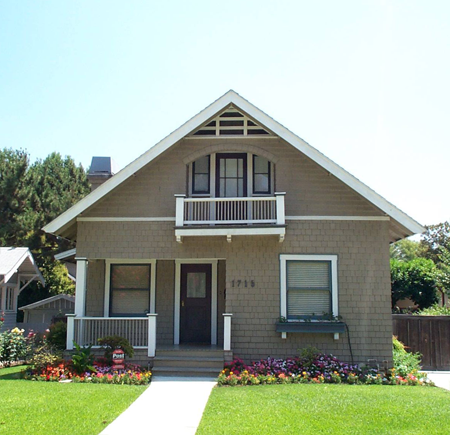
\includegraphics[width=2in]{./Images/house1.png}
        \caption{(\textbf{a})}
    \end{subfigure}
    \begin{subfigure}{2.1in}
        \centering
        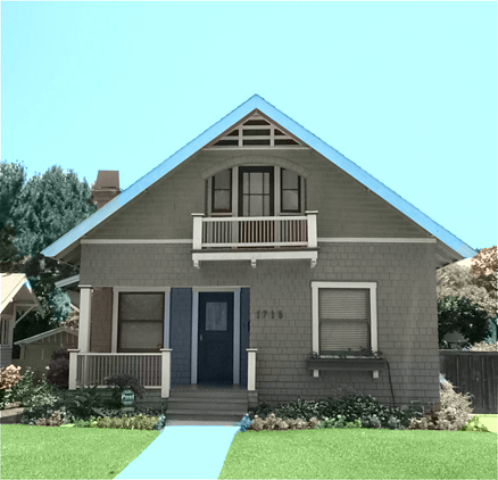
\includegraphics[width=2in]{./Images/house1_colored.png}
        \caption{(\textbf{b})}
    \end{subfigure}
    \begin{subfigure}{2.1in}
        \centering
        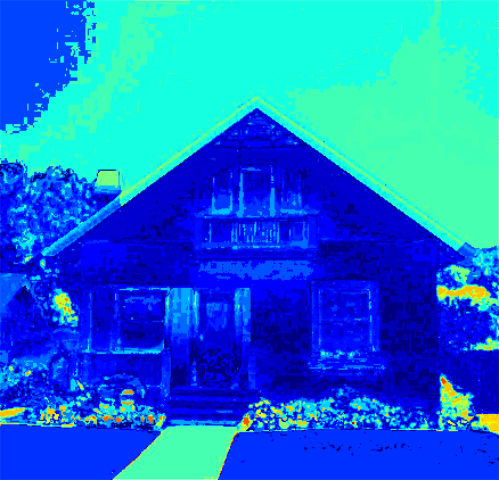
\includegraphics[width=2in]{./Images/house1_acc.png}
        \caption{(\textbf{c})}
    \end{subfigure}
    \begin{subfigure}{2.1in}
        \centering
        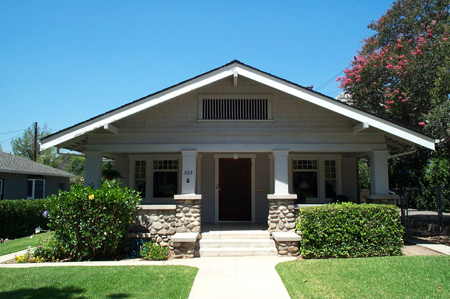
\includegraphics[width=2in]{./Images/house2.png}
        \caption{(\textbf{d})}
    \end{subfigure}
    \begin{subfigure}{2.1in}
        \centering
        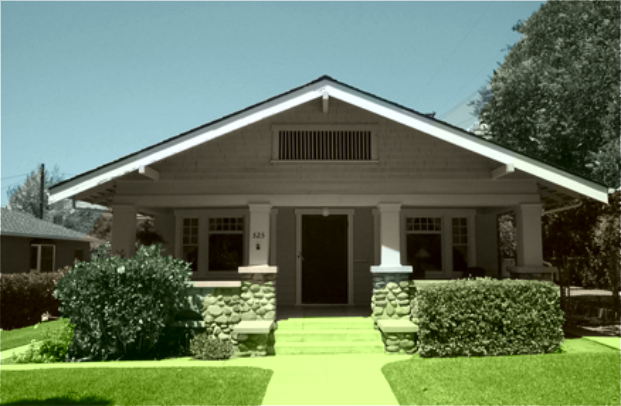
\includegraphics[width=2in]{./Images/house2_colored.png}
        \caption{(\textbf{e})}
    \end{subfigure}
    \begin{subfigure}{2.1in}
        \centering
        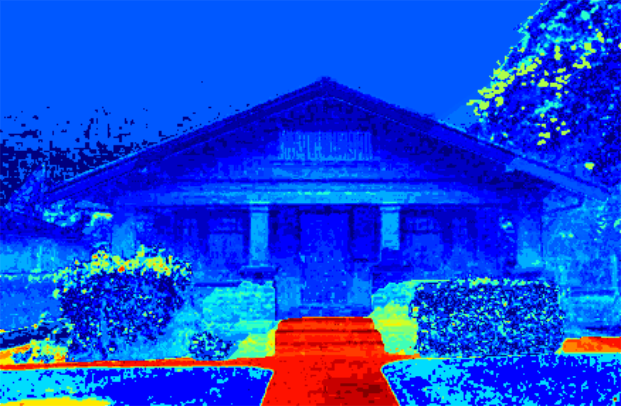
\includegraphics[width=2in]{./Images/house2_acc.png}
        \caption{(\textbf{f})}
    \end{subfigure}
    \caption{Colorizations of house images. (\textbf{a}) Original image of first house. (\textbf{b}) Results from training on \textbf{d} and testing on \textbf{a}. (\textbf{c})  The accuracy of the predicted colors in \textbf{b}. (\textbf{d})  Original image of second house. (\textbf{e})  Results from training on \textbf{a} and testing on \textbf{d}. (\textbf{f})  The accuracy of the predicted colors in \textbf{e}.}
    \label{fig:houses}
\end{figure}

\begin{figure}
    \centering
    \begin{subfigure}{3.5in}
        \centering
        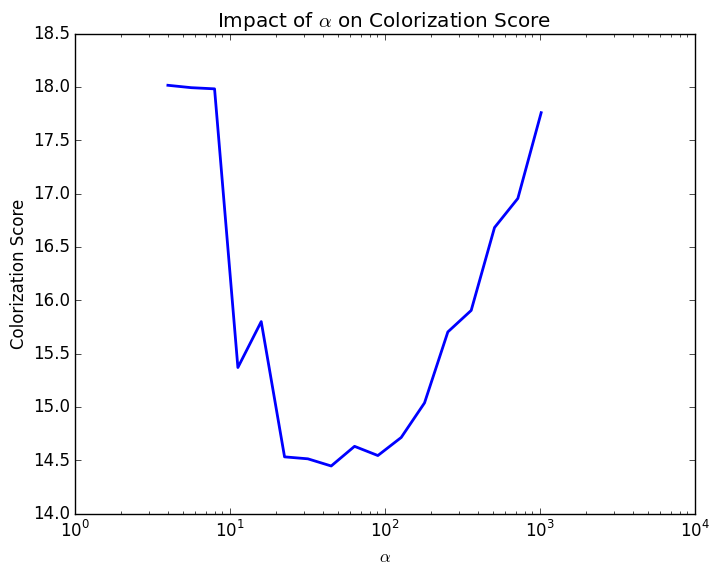
\includegraphics[width=3.4in]{./Images/alpha_graph_house1.png}
        \caption{(\textbf{a})}
    \end{subfigure}
    \begin{subfigure}{3.5in}
        \centering
        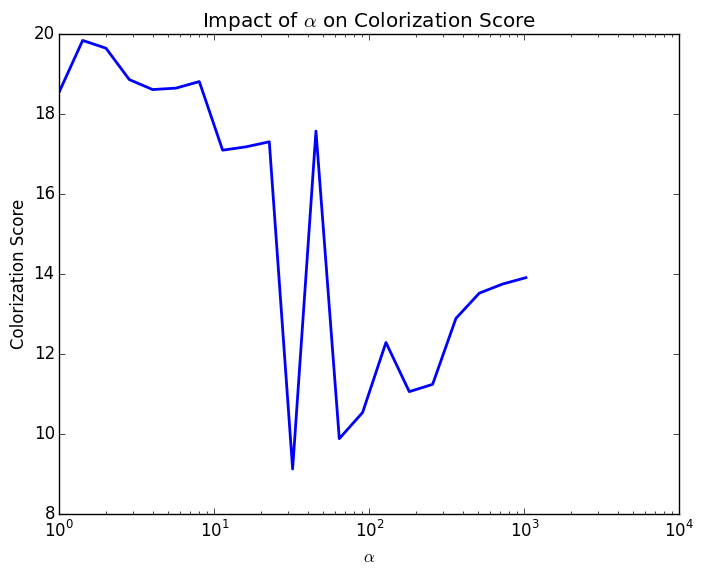
\includegraphics[width=3.4in]{./Images/alpha_graph_mountain.png}
        \caption{(\textbf{b})}
    \end{subfigure}
    \caption{Graphs demonstrating the effect that the $\alpha$ parameter in Equation \ref{eq:energy_min} has on the score of a colorization.  Note that both graphs show that a value from 30 to 60 is optimal. \textbf{(a)} The impact of $\alpha$ on the score when colorizing Figure \ref{fig:houses}(a). \textbf{(b)} The impact of $\alpha$ on the score when colorizing Figure \ref{fig:landscape}(a).}
    \label{fig:alpha_graphs}
\end{figure}

Figure \ref{fig:landscape} shows another set of results from our algorithm.  Note that \ref{fig:landscape}(c) demonstrates a colorization of an image using the same image as the training data.  Understandably, this test achieves the lowest score we've seen on any input, 9.1.  However, we can see that the algorithm performs almost equally well on novel testing data.  We unfortunately do not have access to the original color version of Figure \ref{fig:landscape}(b) and therefore cannot compute a score for this colorization.  Nevertheless, the algorithm's similar behavior on both testing and training data suggests that we have been able to avoid overfitting while constructing our model.  Figure \ref{fig:alpha_graphs}(b) shows the effect of $\alpha$ on the score of the colorization in Figure \ref{fig:landscape}(c).

\begin{figure}
    \centering
    \begin{subfigure}{2.1in}
        \centering
        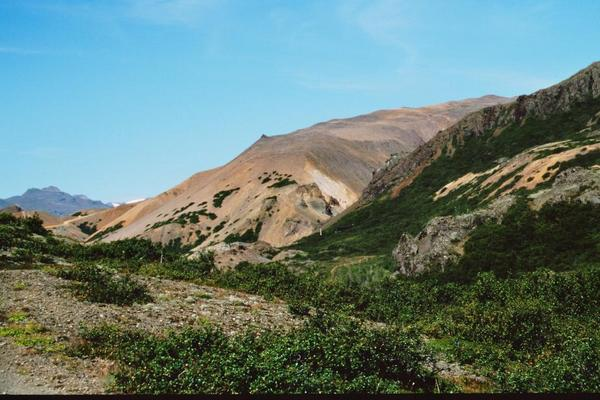
\includegraphics[width=2in]{./Images/mountain_color.jpg}
        \caption{(\textbf{a})}
    \end{subfigure}
    \begin{subfigure}{2.1in}
        \centering
        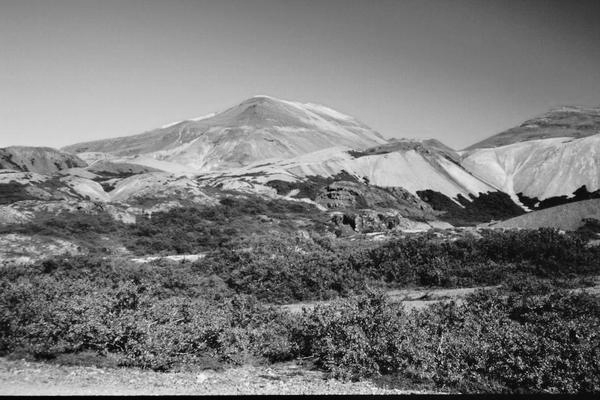
\includegraphics[width=2in]{./Images/mountain_gray.png}
        \caption{(\textbf{b})}
    \end{subfigure}
    \\
    \begin{subfigure}{2.1in}
        \centering
        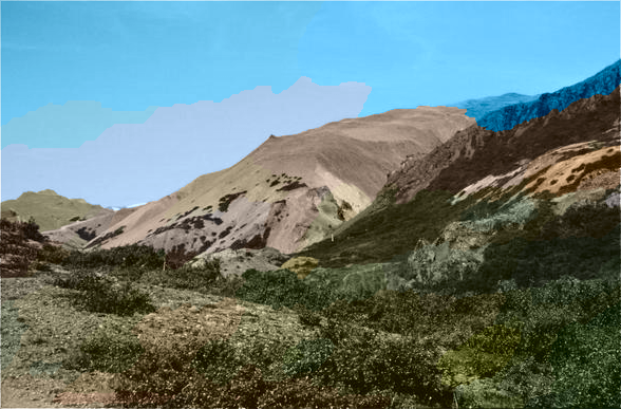
\includegraphics[width=2in]{./Images/mountain_recolored.png}
        \caption{(\textbf{c})}
    \end{subfigure}
    \begin{subfigure}{2.1in}
        \centering
        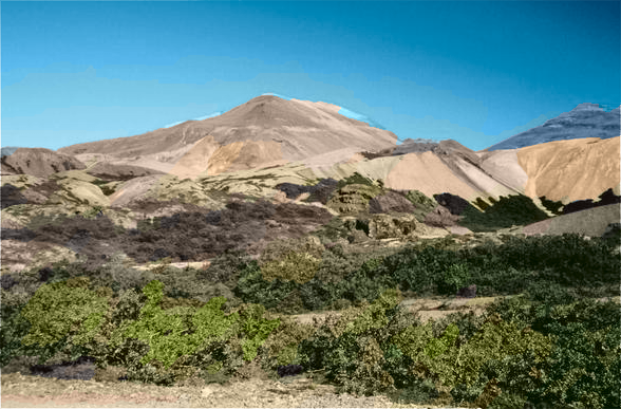
\includegraphics[width=2in]{./Images/mountain_gray_colored.png}
        \caption{(\textbf{d})}
    \end{subfigure}
    \caption{Colorizations of landscape images. (\textbf{a}) Original colored training landscape. (\textbf{b}) Original grayscale testing image. (\textbf{c})  Results from training and testing on \textbf{a}. (\textbf{d}) Results from training on \textbf{a} and testing on \textbf{b}.}
    \label{fig:landscape}
\end{figure}